\fancyhead{}
\fancyfoot{}
\pagestyle{plain}

\lhead{Tecnologías utilizadas}

\chapter{Tecnologías utilizadas}

En este capítulo se presentan las herramientas utilizadas para el desarrollo de este trabajo. En primer lugar, para asegurar que las herramientas seleccionadas sean adecuadas, se realiza una comparación entre alternativas considerando los factores y características más importantes dentro de las actividades.

\section{Componentes de \textit{Hardware}}

Los componentes de hardware abarcan los dispositivos físicos necesarios para la ejecución del sistema, incluyendo microcontroladores, sensores y módulos de comunicación, que se encargan de realizar las tareas físicas y electrónicas requeridas.

\subsection{Placa de Desarrollo WiFi LoRa 32 (V3)}

La \textit{WiFi LoRa 32 (V3)} (véase Figura \ref{fig:heltec}) es una placa de desarrollo \textit{\acrshort{iot-acronym}} basada en el microcontrolador \textit{ESP32-S3FN8}, un procesador de doble núcleo de 32 bits que opera a una frecuencia de hasta 240 MHz. Esta placa está diseñada para aplicaciones de bajo consumo y alto rendimiento en redes inalámbricas, tales como ciudades inteligentes, sistemas de seguridad, agricultura conectada y control industrial. Una de las características principales es la integración de múltiples tecnologías de comunicación, incluyendo \textit{Wi-Fi}, \textit{\gls{ble-glossary} (\acrshort{ble-acronym})} y \textit{\acrshort{lora-acronym}}, lo que le permite ser utilizada en una variedad de entornos \cite{WiFiLoRa32V3}.

La placa cuenta con un transceptor de radio \textit{SX1262}, que permite la transmisión de datos en redes de largo alcance. Soporta modulaciones \textit{\acrshort{lora-acronym}} y \textit{FHSS} para aplicaciones de redes de baja potencia y larga distancia (\textit{LPWAN}), además de la modulación \textit{(G)FSK} para aplicaciones más tradicionales. Este transceptor cubre un rango de frecuencias de 150 MHz a 960 MHz, permitiendo el uso en bandas \textit{ISM} globales. El \textit{SX1262} está diseñado para cumplir con los requisitos de la capa física de la especificación \textit{\acrshort{loraw}} y se ajusta a las regulaciones internacionales de transmisión de radiofrecuencia, lo que lo hace adecuado para su implementación en diversas regiones del mundo \cite{SX1262}.

\begin{figure}[H]
\leavevmode
\begin{minipage}{\textwidth}
\begin{center}
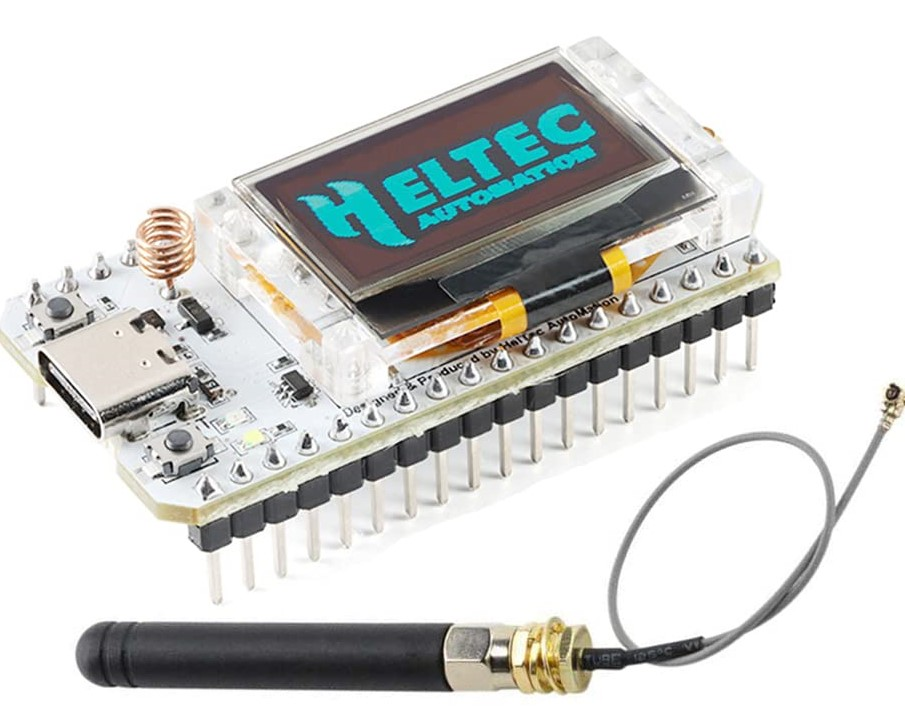
\includegraphics[scale=0.25]{./capitulo_03/figures/HW/Heltec.jpg}
\caption{Placa de desarrollo Heltec\label{fig:heltec}}
\end{center}
\end{minipage}
\end{figure}

La selección de la placa \textit{WiFi LoRa 32 (V3)} para esta investigación se basa en un análisis de diversas placas de desarrollo y herramientas de hardware, con el objetivo de identificar las tecnologías más adecuadas para aplicaciones de \textit{(\acrshort{iot-acronym})}. Se revisaron microcontroladores y transceptores \textit{\acrshort{lora-acronym}}, considerando su funcionalidad y rendimiento.

Según \cite{Cherkaoui2021Review}, los microcontroladores son componentes centrales en la transición de los sistemas embebidos hacia el \textit{\acrshort{iot-acronym}}. Estos dispositivos permiten manejar múltiples procesos de forma autónoma, lo que es esencial para la conectividad y automatización de dispositivos.

Las placas de desarrollo deben cumplir ciertos requisitos fundamentales, como conectividad y compatibilidad con diversas plataformas. En este contexto, se comparan las características clave de tres placas populares: el \textit{Wio E5 Mini}, el \textit{ESP32 Heltec LoRa WiFi V3} y el \textit{NÚCLEO-WL55JC}. Estas placas son reconocidas por su versatilidad y eficiencia en monitoreo y comunicación, como se documenta en diversos estudios \cite{Latifov2023Design, Jengsriwong2023LoRaWAN}.

Con el fin de seleccionar la placa de desarrollo, se establecieron una serie de criterios clave de evaluación que permiten analizar y comparar las opciones disponibles.

\begin{itemize}
    \item \textbf{Conectividad:} Se refiere a la capacidad del dispositivo para soportar diferentes tipos de comunicación y protocolos.
    \item \textbf{Frecuencia \acrshort{lora-acronym}:} Considera la compatibilidad del dispositivo con la frecuencia operativa del protocolo \textit{\acrshort{lora-acronym}} para esta región.
    \item \textbf{Características adicionales:} Incluye funcionalidades extra que pueden mejorar el rendimiento o la versatilidad del dispositivo, como sensores o interfaces de comunicación.
    \item \textbf{Compatibilidad con consolas:} Evalúa qué tan bien la placa puede integrarse con las plataformas de administración y control de dispositivos \textit{\acrshort{loraw}} que permiten la gestión y supervisión del dispositivo.
    \item \textbf{Tamaño/Dimensiones:} Este criterio evalúa la adecuación del tamaño del dispositivo ya que se requiere un diseño compacto.
    \item \textbf{Entornos de desarrollo (Facilidad):} Considera la facilidad de uso del entorno de desarrollo, lo que puede afectar la curva de aprendizaje y el tiempo de implementación.
\end{itemize}

Para reflejar el desempeño relativo de cada dispositivo, se empleó una escala del 1 al 3:

\begin{itemize}
    \item \textbf{3:} Indica el mejor rendimiento o la opción más favorable en ese criterio.
    \item \textbf{2:} Representa un rendimiento intermedio, adecuado pero no el mejor.
    \item \textbf{1:} Refleja un rendimiento limitado en comparación con los otros dispositivos.
\end{itemize}
A continuación, se presenta la tabla \ref{fig:Elec_Mic} comparativa que resume las características técnicas más relevantes de cada dispositivo, facilitando así la selección de la opción más adecuada para este proyecto.

\begin{table}[H]
\centering
\renewcommand{\arraystretch}{1.2} % Ajustar el espacio entre filas
\caption{Tabla comparativa entre Placas de Desarrollo}
\label{fig:Elec_Mic}
\begin{tabular}{|p{4.5cm}|p{1.8cm}|p{3cm}|p{2.6cm}|}
\hline
\textbf{Criterio/Placa}        & \textbf{Wio E5 Mini} & \textbf{ESP32 Heltec WiFi LoRa V3} & \textbf{NÚCLEO-WL55JC} \\ \hline
Conectividad                  &                 2                    & 3                                  & 2                      \\ \hline
Frecuencia LoRa               & 2                    & 3                                  & 3                      \\ \hline
Características adicionales   & 1                    & 3                                  & 1                      \\ \hline
Compatibilidad con consolas   & 3                    & 3                                  & 3                      \\ \hline
Tamaño/Dimensiones            & 3                    & 2                                  & 2                      \\ \hline
Entornos de desarrollo (Facilidad) & 2              & 2                                  & 1                      \\ \hline
\textbf{Total}                & \textbf{13}          & \textbf{16}                        & \textbf{12}            \\ \hline
\end{tabular}
\end{table}


De la tabla comparativa se determina que el \textit{WiFi LoRa V3} es el dispositivo más adecuado para la investigación. Este dispositivo fue seleccionado para las pruebas debido a su equilibrio entre conectividad y compatibilidad con diversos entornos de desarrollo, lo que lo convierte en una opción ideal para la fase de prototipado.


\subsection{Lector RFID MFRC522}

El \textit{MFRC522} (ver Figura \ref{fig:rc522rf}) es un circuito integrado de alto rendimiento diseñado para la lectura y escritura de tarjetas de identificación por radiofrecuencia (\textit{\acrshort{rfid-acronym}}) a 13.56 MHz, compatible con los estándares ISO/IEC 14443 A y tecnologías \textit{MIFARE} y \textit{NTAG}. Este módulo es ideal para aplicaciones de control de acceso, sistemas de pago sin contacto, y sistemas de seguimiento por identificación de objetos, brindando un diseño compacto y eficiente.

El \textit{MFRC522} está equipado con un transmisor integrado que permite la comunicación con tarjetas \textit{\acrshort{rfid-acronym}} sin necesidad de circuitos adicionales, proporcionando una distancia de operación de hasta 50 mm (dependiendo del diseño y tamaño de la antena) \cite{MFRC522Datasheet}. 

\begin{figure}[H]
\leavevmode
\begin{minipage}{\textwidth}
\begin{center}
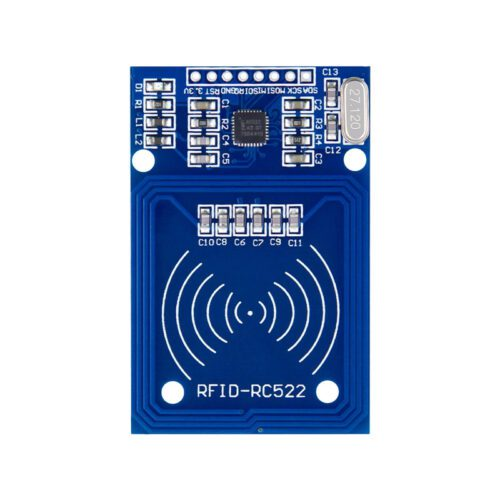
\includegraphics[scale=0.35]{./capitulo_03/figures/HW/rc522.jpg}
\caption{Lector \textit{\acrshort{rfid-acronym}} \label{fig:rc522rf}}
\end{center}
\end{minipage}
\end{figure}

En el ámbito de los sistemas de control de acceso basados en \textit{\acrshort{rfid-acronym}}, diversos trabajos han explorado el uso de estas tecnologías por su facilidad de implementación y capacidad para integrarse en proyectos de \textit{\acrshort{iot-acronym}} y seguridad. Por ejemplo, investigaciones previas \cite{Cherkaoui2021Review, Latifov2023Design} resaltan la viabilidad y flexibilidad de los módulos \textit{\acrshort{rfid-acronym}} en, aplicaciones prácticas.

Para la selección del módulo \textit{\acrshort{rfid-acronym}} más adecuado para el presente proyecto, se consideraron criterios clave como la disponibilidad en el mercado, el costo, la simplicidad de implementación y la compatibilidad con plataformas de desarrollo comunes. A continuación, se presenta la tabla comparativa \ref{fig:tablaRFID}, que incluye tres módulos \textit{\acrshort{rfid-acronym}}: \textit{PN532 NFC RFID Module V3}, \textit{RC522 RFID Module} y \textit{R200 UHF RFID Reader}.

\begin{table}[H]
\centering
\renewcommand{\arraystretch}{1.2} % Ajusta el espacio entre filas
\caption{Tabla comparativa entre módulos \textit{\acrshort{rfid-acronym}}}
\label{fig:tablaRFID}
\begin{tabular}{|p{4.5cm}|p{2.5cm}|p{2.5cm}|p{2.5cm}|}
\hline
\textbf{Criterio / Módulos}                 & \textbf{PN532 NFC RFID Module V3} & \textbf{RC522 RFID Module} & \textbf{R200 UHF RFID Reader} \\ \hline
Disponibilidad en el mercado               & 2                                & 3                          & 1                              \\ \hline
Costo                                      & 2                                & 3                          & 1                              \\ \hline
Simplicidad de implementación              & 2                                & 3                          & 1                              \\ \hline
Compatibilidad con plataformas populares   & 2                                & 3                          & 1                              \\ \hline
Adecuación para pruebas y prototipado      & 2                                & 3                          & 1                              \\ \hline
\textbf{Total}                             & \textbf{10}                      & \textbf{15}                & \textbf{6}                     \\ \hline
\end{tabular}
\end{table}


De acuerdo con los resultados obtenidos en la tabla comparativa, el \textit{RC522 RFID Module} ha sido seleccionado como la opción más adecuada para el proyecto en curso. Su alta disponibilidad, bajo costo y facilidad de implementación lo convierten en el candidato ideal para llevar a cabo pruebas y prototipos. Además, su compatibilidad con plataformas populares como \textit{Arduino} y su sencilla integración en sistemas de control de acceso lo destacan frente a los otros módulos evaluados.

En contraste, aunque el \textit{PN532} ofrece características avanzadas como la compatibilidad \textit{NFC}, su implementación es más compleja. El \textit{R200 UHF}, aunque destaca por su capacidad de lectura a larga distancia, es menos apropiado para un proyecto de bajo costo y prototipado rápido debido a su precio más elevado y la necesidad de antenas externas.

\subsection{Módulo GNSS GP-02 Kit}

El \textit{GP-02-Kit} (ver Figura \ref{fig:gnssgp}) es un módulo de desarrollo altamente integrado que incorpora un receptor de navegación por satélite multimodo de alto rendimiento. El módulo utiliza el chip de posicionamiento por satélite \textit{AT6558R}, el cual combina un frontal de radiofrecuencia, un procesador de banda base digital, una CPU \textit{RISC} de 32 bits, gestión de energía y funciones de detección y protección de antenas activas.

\begin{figure}[H]
\leavevmode
\begin{minipage}{\textwidth}
\begin{center}
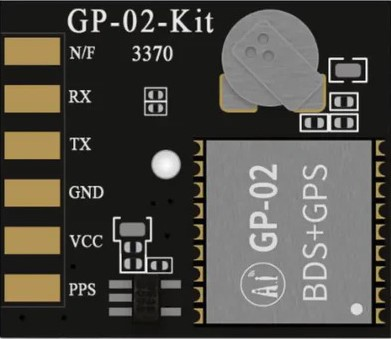
\includegraphics[scale=0.5]{./capitulo_03/figures/HW/GP-02.jpg}
\caption{Módulo de desarrollo \textit{GP-02 Kit} \label{fig:gnssgp}}
\end{center}
\end{minipage}
\end{figure}

Este módulo es compatible con múltiples sistemas de navegación por satélite, incluyendo el sistema de navegación por satélite \textit{BeiDou} de China, el sistema \textit{\acrshort{gps-acronym}} de Estados Unidos y el \textit{GLONASS} de Rusia, lo que le permite realizar un posicionamiento conjunto multi-sistema, garantizando alta precisión en aplicaciones críticas de geolocalización.

El \textit{GP-02-Kit} sigue el protocolo \textit{NMEA} para la transmisión de datos y se comunica con otros dispositivos a través de una interfaz serial \textit{\acrshort{uart-acronym}}, la cual soporta tasas de transferencia de hasta 256000 bps. Además, cuenta con una antena cerámica integrada, lo que simplifica su uso en entornos móviles o aplicaciones de seguimiento donde el tamaño y la eficiencia son esenciales \cite{GP02Kit2021}.

\subsection{Placa de Desarrollo ESP-WROOM-32}

El \textit{ESP32-WROOM-32} (ver Figura \ref{fig:wrom32}) es un módulo \textit{MCU} de alto rendimiento que incluye \textit{Wi-Fi}, \textit{BT} y \textit{\acrshort{ble-acronym}}, ideal para una variedad de aplicaciones, desde redes de sensores de bajo consumo hasta tareas avanzadas como codificación de voz, transmisión de música y decodificación de \textit{MP3}.

En el núcleo de este módulo se encuentra el chip \textit{ESP32-D0WDQ6*}, diseñado para ofrecer escalabilidad y flexibilidad. Posee dos núcleos de \textit{CPU}, controlables individualmente, con una frecuencia de reloj ajustable entre 80 MHz y 240 MHz. Además, permite apagar la \textit{CPU} principal y usar el coprocesador de bajo consumo para monitorear los periféricos de forma constante. Entre sus múltiples periféricos, el \textit{ESP32} integra sensores táctiles capacitivos, sensores \textit{Hall}, interfaz para tarjeta \textit{SD}, \textit{Ethernet}, \textit{\acrshort{spi-acronym}} de alta velocidad, \textit{\acrshort{uart-acronym}}, \textit{\acrshort{i2s-acronym}} e \textit{\acrshort{i2c-acronym}} \cite{Espressif2019}.

Este microcontrolador fue elegido debido a su flexibilidad y disponibilidad, así como por sus capacidades de manejo de periféricos y transmisión de datos, lo que lo convierte en una opción adecuada para las demandas de comunicación en este sistema.

\begin{figure}[H]
\leavevmode
\begin{minipage}{\textwidth}
\begin{center}
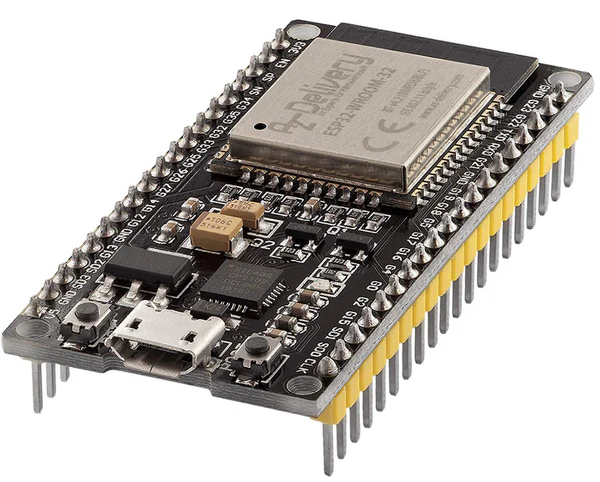
\includegraphics[scale=0.3]{./capitulo_03/figures/HW/wroomp.png}
\caption{Placa de desarrollo \textit{ESP32} \label{fig:wrom32}}
\end{center}
\end{minipage}
\end{figure}


\section{Componentes de \textit{Software}}
Los componentes de software proporcionan las herramientas y entornos de programación necesarios para diseñar, compilar y cargar el código en el hardware. Además, facilitan la visualización de los datos recolectados, permitiendo una supervisión eficiente y en tiempo real del sistema. No solo posibilitan la integración con el hardware, sino que también proporciona una plataforma para interpretar y presentar la información
\subsection{\textit{Helium Console}}
Helium Console es una plataforma desarrollada por Helium que permite la gestión de organizaciones y dispositivos en redes \acrshort{loraw}  a través de una interfaz basada en navegador web. Actúa como un servidor de red \acrshort{loraw} (\acrshort{lns-acronym}, por sus siglas en inglés, \gls{lns-glossary}) compatible con la blockchain de Helium, conocido como Router, que facilita la comunicación entre dispositivos \acrshort{loraw} y la red de Helium. Helium Console simplifica la integración y operación de dispositivos, proporcionando a los usuarios una forma eficiente y directa de administrar sus dispositivos \acrshort{iot-acronym} (Internet of Things, o Internet de las Cosas) dentro de la infraestructura de la red Helium \cite{heliumDocs}.

Una de las principales ventajas de Helium Console es su enfoque “plug-and-play” (lista para usar), lo que significa que los usuarios pueden configurar y operar su propia Organización Única de Identificación (OUI, Organizationally Unique Identifier) en la red Helium de manera rápida y sin necesidad de permisos especiales. Dado que la red de Helium es descentralizada y abierta, la operación de una OUI es completamente permissionless (sin necesidad de permisos), lo que facilita la incorporación de nuevos dispositivos \acrshort{iot-acronym} sin las barreras típicas que se encuentran la mayoria de redes.

Se evaluaron varias plataformas de servidor de red \acrshort{loraw} (\acrshort{lns-acronym}) con el objetivo de elegir la más adecuada para el trabajo. El proceso de selección se basó en analizar criterios específicos que afectan directamente la funcionalidad y adaptabilidad de cada plataforma a los requisitos del proyecto.
\\
Criterios considerados
\begin{itemize}

\item Costo: Considera el gasto involucrado en utilizar la plataforma, desde suscripciones hasta la infraestructura adicional que pueda requerirse. Cuanto menor es el costo, mejor es la evaluación.

\item Facilidad de Uso: Mide la simplicidad y accesibilidad de la interfaz y su curva de aprendizaje, ideal para usuarios con diversos niveles de experiencia.

\item Escalabilidad: Evalúa la capacidad de la plataforma para adaptarse y crecer, tanto en usuarios como en dispositivos, sin que el rendimiento disminuya.

\item Cobertura: Analiza la disponibilidad geográfica de la plataforma y su cobertura en distintas áreas.

\item Control y Personalización: Valora el nivel de control que ofrece la plataforma para adaptar la infraestructura y configuraciones específicas.

\item Privacidad y Seguridad: Mide las medidas de seguridad y cifrado en la transmisión de datos. Mayor puntaje si la plataforma ofrece seguridad avanzada y privacidad de datos.

\item Integración: Evalúa la facilidad de integración de la plataforma con otros sistemas y su capacidad para conectarse con tecnologías \acrshort{iot-acronym}.

\item Documentación: Analiza la calidad y accesibilidad de la documentación proporcionada, indispensable para configurar la plataforma.
 
\end{itemize}

En la tabla \ref{fig:Elec_lns} se comparan plataformas de servidor de red \acrshort{loraw} (\acrshort{lns-acronym}) como: Helium Console, The Things Network (TTN), ChirpStack, Loriot para determinar la plataforma más adecuada.

%\usepackage{tabularx} % Asegúrate de incluir este paquete en el preámbulo
\begin{table}[H]
\centering
\renewcommand{\arraystretch}{1.33} % Ajusta el espacio entre filas
\caption{Comparativa de plataformas LoRaWAN}
\label{fig:Elec_lns}
\begin{tabular}{|p{3cm}|p{2.5cm}|p{2.3cm}|p{2.2cm}|p{1.7cm}|}
\hline
\textbf{Criterios} & \textbf{Helium Console} & \textbf{The Things Network (TTN)} & \textbf{ChirpStack} & \textbf{Loriot} \\ \hline
Costo             & Bueno                   & Excelente                         & Bueno              & Bueno          \\ \hline
Facilidad de Uso  & Excelente               & Excelente                         & Regular            & Excelente      \\ \hline
Escalabilidad     & Excelente               & Regular                           & Bueno              & Bueno          \\ \hline
Cobertura         & Bueno                   & Bueno                             & Regular            & Bueno          \\ \hline
Control y Personalización & Regular        & Regular                           & Excelente          & Bueno          \\ \hline
Privacidad y Seguridad    & Bueno          & Regular                           & Excelente          & Excelente      \\ \hline
Integraciones     & Excelente               & Excelente                         & Excelente          & Bueno          \\ \hline
Documentación     & Excelente               & Excelente                         & Regular            & Excelente      \\ \hline
\end{tabular}
\end{table}


Helium Console destaca principalmente como la opción ganadora debido a su cobertura, un aspecto crucial en el análisis comparativo. Aunque otras plataformas ofrecen excelentes características en varias áreas, Helium sobresale por su capacidad de brindar una red descentralizada y global. Además, otras características como su facilidad de uso, integraciones y documentación excelente también refuerzan su posición.

\subsection{Thingsboard}
ThingsBoard es una plataforma \acrshort{iot-acronym} de código abierto que facilita la recopilación, procesamiento, visualización y  gestión de dispositivos de datos. La plataforma destaca por su capacidad para manejar grandes volúmenes de datos y dispositivos, lo que la convierte en una opción robusta y flexible para diversas aplicaciones en el ámbito de la Internet de las Cosas. Su diseño modular permite a los desarrolladores integrar y gestionar dispositivos de forma eficiente, sin necesidad de construir una infraestructura desde cero.

La arquitectura de ThingsBoard es clave para su funcionalidad, y se puede implementar en dos modalidades: monolítica y microservicios. En su modo monolítico, todos los componentes se ejecutan dentro de una única máquina virtual Java (JVM), optimizando el uso de recursos del sistema operativo y simplificando su implementación en entornos con limitaciones de memoria y procesamiento. Este enfoque centralizado facilita el desarrollo y el prototipado de soluciones \acrshort{iot-acronym}, al requerir menos configuración y memoria. Por otro lado, la modalidad basada en microservicios distribuye los componentes del sistema en nodos independientes, lo que permite una escalabilidad horizontal y una mayor tolerancia a fallos, ideal para proyectos de gran escala donde es crucial gestionar grandes cantidades de dispositivos y datos de manera eficiente. 
La figura \ref{fig:tbarqui} ilustra cómo ThingsBoard organiza sus componentes y cómo interactúan para manejar la comunicación entre dispositivos y sistemas externos \cite{ThingsBoard}.

\begin{figure}[H]
\leavevmode
\begin{minipage}{\textwidth}
\begin{center}
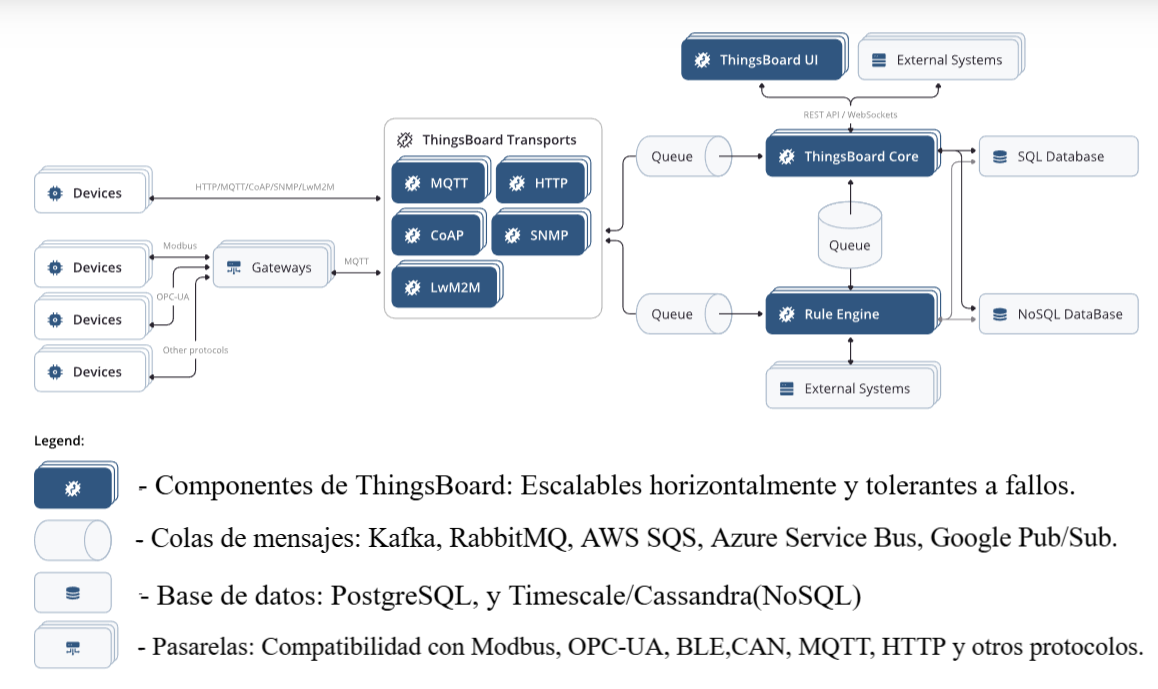
\includegraphics[width=1.0\textwidth]{./capitulo_03/figures/SW/tbarquitecture.png}
\caption{Diagrama de Arquitectura ThingsBoard\label{fig:tbarqui}}
\end{center}
\end{minipage}
\end{figure}

Uno de los componentes esenciales de ThingsBoard es su motor de reglas (Rule Engine), que juega un papel central en la automatización y procesamiento de eventos dentro de la plataforma. Este motor permite procesar los datos entrantes desde los dispositivos \acrshort{iot-acronym} y ejecutar acciones automáticas basadas en la lógica definida por el usuario. El sistema procesa los datos a través de una serie de nodos que realizan diferentes operaciones, como almacenamiento, generación de alertas o control remoto de dispositivos mediante llamadas a procedimientos remotos RPC. Esto posibilita la creación de flujos de trabajo complejos que reaccionan en tiempo real a los eventos generados por los dispositivos, permitiendo a la plataforma tomar decisiones y ejecutar acciones automáticamente sin intervención humana. 
En la Figura \ref{fig:ruleengine} , donde se puede observar cómo se configuran las cadenas de reglas para tomar decisiones basadas en los mensajes recibidos, por ejemplo, enviando comandos de RPC o almacenando datos en bases de datos \cite{ThingsBoard}.

\begin{figure}[H]
\leavevmode
\begin{minipage}{\textwidth}
\begin{center}
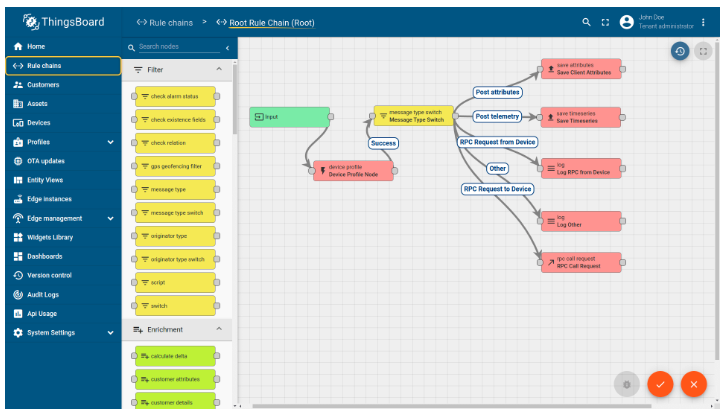
\includegraphics[width=\textwidth]{./capitulo_03/figures/SW/ruleengine.png}
\caption{Cadena de reglas raíz ThingsBoard\label{fig:ruleengine}}
\end{center}
\end{minipage}
\end{figure}

Una visualización adecuada de los datos adquiridos es esencial ya facilita el procesamiento de los mismos, lo que contribuye a la precisión y efectividad de las decisiones tomadas a partir de esta información.  Con el objetivo de facilitar esta visualización y gestión de datos, se seleccionó una plataforma \acrshort{iot-acronym}, basándose en estudios que resaltan el uso de estas herramientas en contextos de monitoreo y análisis de datos \cite{Alquhali2019IOT, Nwankwo2022IoT-Assisted, Santa2019LPWAN-Based, Suwaid2019Embedded, Alavi2019State, K2023IoT}. 

Para determinar la plataforma más adecuada, se evaluaron Ubidots, ThingSpeak y ThingsBoard bajo criterios técnicos relevantes para entornos de prototipado, incluyendo:


\begin{itemize}
    \item Escalabilidad: Este criterio evaluó la capacidad de cada plataforma para manejar un aumento en el número de dispositivos y datos a medida que el proyecto crece.

    \item Protocolos Soportados: Se analizó la diversidad de protocolos de comunicación \acrshort{iot-acronym} que cada plataforma puede gestionar.

    \item Visualización de Datos: Este criterio evaluó la calidad de las herramientas de visualización de datos disponibles en cada plataforma.

    \item Automatización de Reglas: Se evaluó la capacidad de cada plataforma para configurar reglas y flujos de trabajo automáticos.

    \item Costo: Este criterio consideró los costos asociados al uso de las plataformas. 

    \item Soporte y Comunidad: La disponibilidad de soporte técnico y la existencia de una comunidad activa fueron evaluadas. 

    \item Instalación Local (On-Premise): Este criterio evaluó la opción de implementar la plataforma en un servidor propio.

    \item Facilidad de Uso: Finalmente, se evaluó la intuitividad y facilidad de uso de la interfaz para usuarios tanto novatos como avanzados.
\end{itemize}

Cada plataforma fue calificada en una escala de 1 a 3, permitiendo una comparación cuantitativa de sus capacidades, donde:
\begin{itemize}
    \item 1 indica un rendimiento bajo.
    \item 2 un rendimiento medio.
    \item 3 un rendimiento alto.
\end{itemize}

La tabla \ref{fig:Elec_tb} resume los resultados obtenidos, y constituye la base para seleccionar la plataforma que mejor responde a los requerimientos de visualización y control de datos en el proyecto.

\begin{table}[H]
\centering
\renewcommand{\arraystretch}{1.3} % Ajusta el espacio entre filas
\caption{Tabla comparativa de Plataformas IoT}
\label{fig:Elec_tb}
\begin{tabularx}{\textwidth}{|p{4.4cm}|X|X|X|}
\hline
\textbf{Criterio/Plataforma}                & \textbf{Ubidots} & \textbf{ThingSpeak} & \textbf{ThingsBoard} \\ \hline
 Escalabilidad                           & 2                & 2                   & 3                    \\ \hline
 Protocolos Soportados                   & 2                & 2                   & 3                    \\ \hline
 Visualización de Datos                  & 3                & 2                   & 3                    \\ \hline
 Automatización de Reglas                & 2                & 2                   & 3                    \\ \hline
 Costo                                   & 3                & 3                   & 3                    \\ \hline
 Soporte y Comunidad                     & 3                & 3                   & 3                    \\ \hline
 Instalación Local (On-Premise)          & 1                & 1                   & 3                    \\ \hline
 Facilidad de Uso                        & 3                & 3                   & 3                    \\ \hline
\textbf{Total}                             & \textbf{17}      & \textbf{16}         & \textbf{21}          \\ \hline
\end{tabularx}
\end{table}


De acuerdo con los criterios evaluados, ThingsBoard se destaca como la plataforma \acrshort{iot-acronym} más adecuada para el presente proyecto. Su versión Community Edition permite una instalación local sin costos asociados, lo cual resulta especialmente ventajoso en un entorno de prototipado. Además, su capacidad para escalar y su soporte para una amplia gama de protocolos lo convierten en una opción robusta para gestionar y visualizar información en tiempo real. Una de las razones clave para elegir ThingsBoard fue su integración nativa con MQTT \cite{MQTT}, un protocolo ligero que utiliza un modelo de publicación/suscripción para optimizar la transmisión de datos entre dispositivos \acrshort{iot-acronym}. Esto permite una comunicación eficiente, en tiempo real y con bajo consumo de recursos, asegurando la escalabilidad del sistema. Estas características, junto con la posibilidad de uso gratuito y sin limitaciones de licenciamiento comercial, posicionan a ThingsBoard como la solución óptima, permitiendo una implementación sostenible y adaptable.








\subsection{Arduino IDE}

El Arduino IDE o Entorno de Desarrollo Integrado de Arduino, es un entorno de desarrollo integrado que facilita la programación y carga de código en microcontroladores mediante una interfaz amigable \cite{ArduinoIDE}. Permite a los usuarios escribir y editar “sketches” (programas o códigos) en un lenguaje basado en C/C++, simplificado para el control de hardware, lo que agiliza el desarrollo de proyectos de electrónica.

Una de sus ventajas es la flexibilidad en la configuración de hardware, gracias a su “Gestor de Placas” que adapta el código a distintos modelos de microcontroladores y permite la instalación de librerías adicionales. En este proyecto, el Arduino IDE es especialmente útil debido a su compatibilidad con la placa Heltec LoRa WiFi 32 V3, que cuenta con librerías y referencias específicas de Heltec, lo que simplifica la integración de \textit{\acrshort{loraw}} y WiFi.

Además, el IDE permite la carga del código de manera directa desde una conexión USB o inalámbrica, haciendo más ágil el ciclo de pruebas y depuración, gracias a sus herramientas básicas para detectar errores en el código. Estas características hacen del Arduino IDE una opción versátil y eficiente para proyectos con microcontroladores, adecuada para usuarios de todos los niveles.

La interfaz del Arduino IDE se muestra en la Figura \ref{fig:arduino_ide}, donde es posible observar sus principales herramientas para la edición y carga de código.

\begin{figure}[H]
\leavevmode
\begin{minipage}{\textwidth}
\begin{center}
    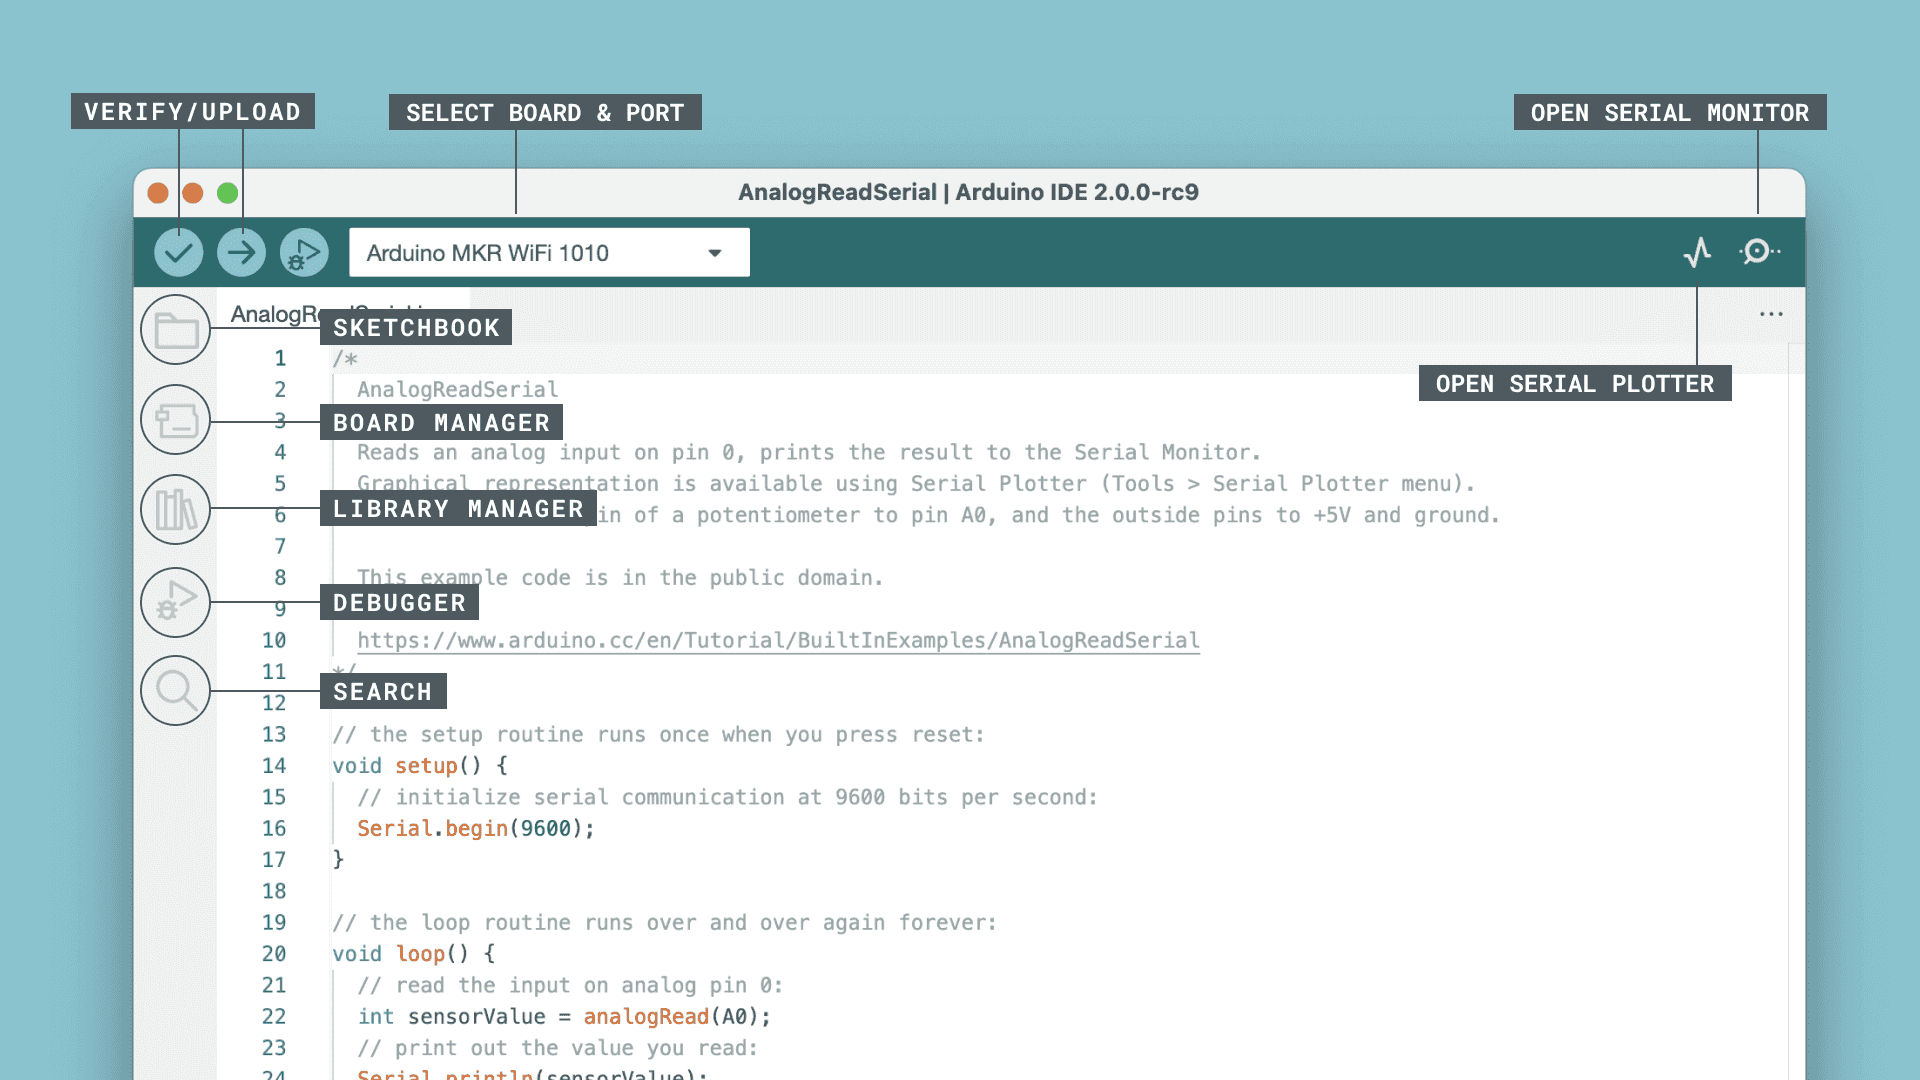
\includegraphics[width=1.0\textwidth]{./capitulo_03/figures/SW/ide-2-ino.png} % Ajusta el tamaño y la ruta de la imagen
    \caption{Interfaz del Arduino IDE 2\cite{ArduinoIDEImage}.}
    \label{fig:arduino_ide}
\end{center}
\end{minipage}
\end{figure}


\subsection{Fritzing}
Fritzing es un software de automatización del diseño electrónico (Electronic Design Automation, EDA) orientado a diseñadores, artistas, investigadores y cualquier persona interesada en la electrónica y el desarrollo de prototipos. Su propósito principal es ofrecer herramientas que faciliten la documentación y el intercambio de proyectos, permitiendo a los usuarios crear y diseñar circuitos de forma visual y accesible \cite{FritzingSoftware}.

El programa se destaca por su interfaz intuitiva, que permite a los usuarios diseñar circuitos, crear esquemas de circuitos impresos y compartir sus prototipos. Además, Fritzing es compatible con otras herramientas de diseño como Processing y Arduino, formando un ecosistema en el que los usuarios pueden documentar y compartir sus proyectos con facilidad. Esto lo convierte en una herramienta valiosa tanto para la enseñanza de electrónica como para la creación de prototipos destinados a la fabricación \cite{FritzingPrimerosPasos}.

La Figura \ref{fig:fritzingf} muestra la interfaz de Fritzing, en la cual es posible visualizar y editar circuitos de manera sencilla y gráfica. Este entorno facilita tanto el diseño de circuitos como la creación de esquemas listos para fabricación, adaptándose a las necesidades de diversos usuarios y proyectos.

\begin{figure}[H]
\leavevmode
\begin{minipage}{\textwidth}
\begin{center}
    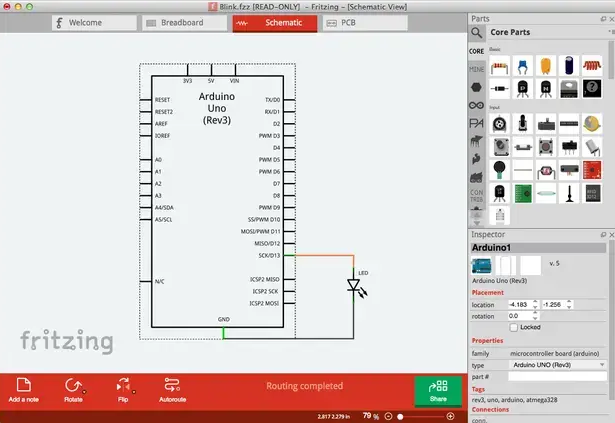
\includegraphics[width=0.7\textwidth]{./capitulo_03/figures/SW/fritzing.png} % Ajusta el tamaño y la ruta de la imagen
    \caption{Entorno de diseño de Fritzing mostrando el esquema de una placa\cite{FritzingPrimerosPasos}.}
    \label{fig:fritzingf}
\end{center}
\end{minipage}
\end{figure}



\subsection{Blender}

Blender es una suite de creación 3D gratuita y de código abierto que soporta toda la cadena de producción 3D: modelado, rigging, animación, simulación, renderizado, composición, seguimiento de movimiento, edición de video e incluso creación de juegos. Los usuarios avanzados pueden utilizar la \acrshort{api-acronym} de Blender para scripting en Python, permitiendo personalizar la aplicación y desarrollar herramientas especializadas que a menudo se incluyen en futuras versiones.

Una de las grandes ventajas de Blender es su accesibilidad y versatilidad. Al ser gratuito y estar disponible para múltiples plataformas como Linux, Windows y macOS, permite que tanto individuos como pequeños estudios accedan a herramientas profesionales sin incurrir en altos costos. Su interfaz unificada y el uso de OpenGL garantizan una experiencia consistente en todos los sistemas operativos \cite{Blender}.

Además, Blender es impulsado por una comunidad activa bajo la Licencia Pública General de GNU (GPL), lo que significa que cualquier persona puede contribuir al desarrollo del software. Esto conduce a la incorporación constante de nuevas funciones, correcciones rápidas de errores y mejoras en la usabilidad. La colaboración comunitaria fomenta la innovación y asegura que el software evolucione para satisfacer las necesidades cambiantes de sus usuarios \cite{Blender1}.

Blender no solo ofrece una solución completa para la creación de contenido 3D, sino que también promueve un entorno colaborativo y abierto. Su combinación de potencia, flexibilidad y gratuidad lo convierte en una opción ideal para aquellos que buscan desarrollar proyectos creativos sin las limitaciones de los software propietarios.

 En la figura \ref{fig:blender}, se muestra la interfaz de Blender, donde es posible dibujar directamente en una ventana gráfica 3D. Esta funcionalidad abre una libertad de flujo de trabajo sin igual para creadores de guiones gráficos y artistas 2D. Blender permite combinar elementos 2D y 3D directamente en la ventana gráfica. Además, incluye capas y colores para trazos y rellenos, así como la capacidad de esculpir pinceladas y asociarlas a objetos 3D.


 \begin{figure}[H]
\leavevmode
\begin{minipage}{\textwidth}
\begin{center}
    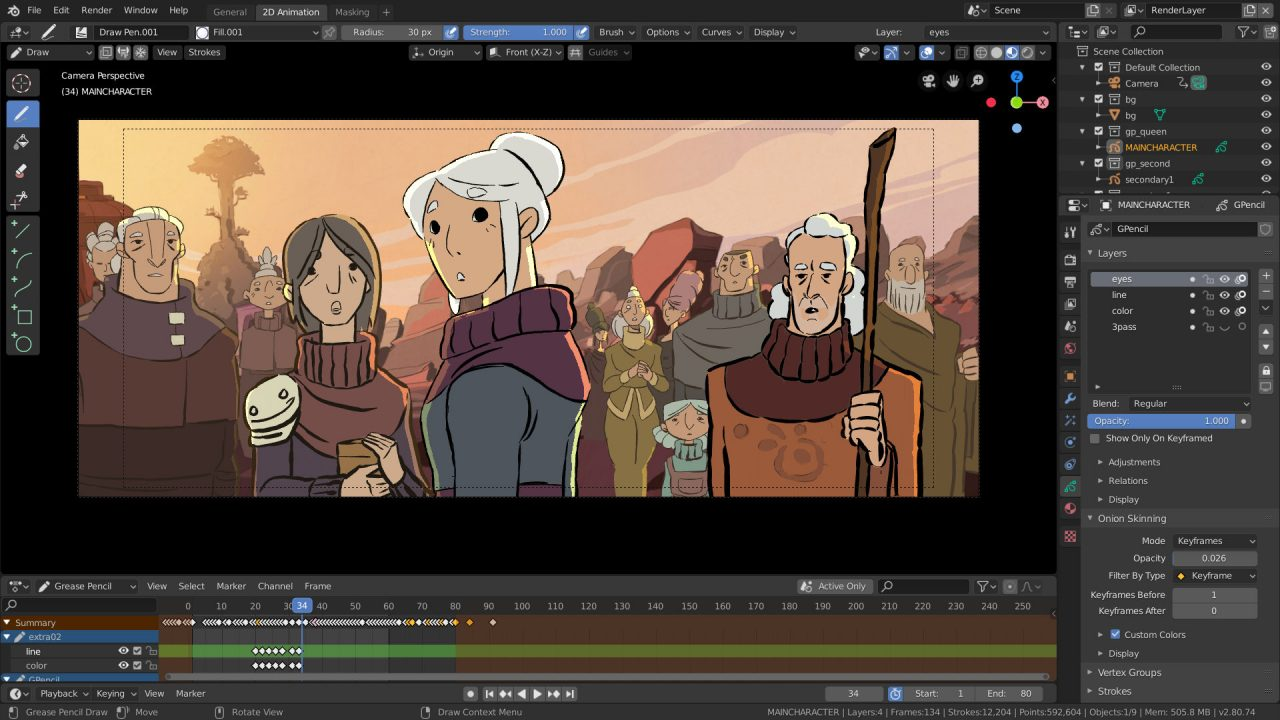
\includegraphics[width=0.7\textwidth]{./capitulo_03/figures/SW/herojpg.jpg} % Ajusta el tamaño y la ruta de la imagen
    \caption{Entorno de desarrollo en Blender.}
    \label{fig:blender}
\end{center}
\end{minipage}
\end{figure}